% *********************************************************************
% © 2021 Jeremy Sylvestre
%
% Permission is granted to copy, distribute and/or modify this document
% under the terms of the GNU Free Documentation License, Version 1.3 or
% any later version published by the Free Software Foundation; with no
% Invariant Sections, no Front-Cover Texts, and no Back-Cover Texts. A
% copy of the license is included in the appendix entitled “GNU Free
% Documentation License” that appears in the output document of this
% PreTeXt source code. All trademarks™ are the registered® marks of
% their respective owners.
%
% *********************************************************************

\newcommand*{\xmin}{-0.5}
\newcommand*{\xmax}{4}
\newcommand*{\ymin}{-0.5}
\newcommand*{\ymax}{8}

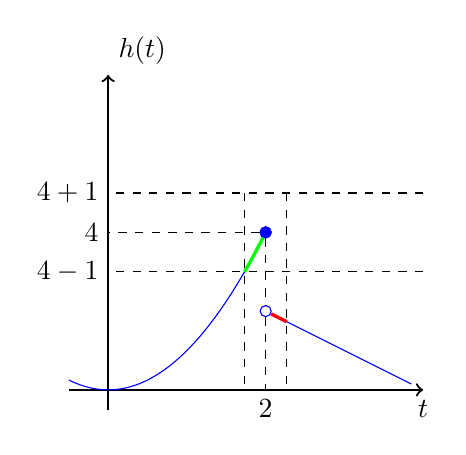
\begin{tikzpicture}
[
	closedpt/.style={circle,draw,fill,inner sep=0pt,minimum size=4pt},
	openpt/.style={circle,draw,inner sep=0pt,minimum size=4pt},
	yscale=0.5
]

	% axes
	\draw[->,thick] (\xmin,0) -- (\xmax,0) node[below] {$t$};
	\draw[->,thick] (0,\ymin) -- (0,\ymax) node[above right] {$h(t)$};

	\node[closedpt,blue] at (2,4) (p) {};
	\node[openpt,blue] at (2,2) (l) {};

	\draw[dashed] (p) -- (0,4) node[left] {$4$};

	\draw[dashed] (\xmax,3) -- (0,3) node[left] {$4 - 1$};
	\draw[dashed] (\xmax,5) -- (0,5) node[left] {$4 + 1$};

	\draw[dashed] (1.732,5) -- (1.732,0);
	\draw[dashed] (2.268,5) -- (2.268,0);

	% graph
	\draw[blue, domain=-0.5:2, smooth] plot (\x,{\x * \x});
	\draw[very thick, green, domain=1.732:2, smooth] plot (\x,{\x * \x});

	\draw[dashed] (p) -- (l) -- (2,0) node[below] {$2$};
	\draw[blue] (l) -- (3.85,0.15);

	\draw[very thick, red] (l) -- (2.268,1.732);

	\node[closedpt,blue] at (2,4) (p) {};

\end{tikzpicture}
